\section[Preconditioning]{The influence of preconditioning on MHD magnetospheric
models} This section addresses the influence of the amount of time spent on preconditioning
on magnetospheric MHD models. There are examples of previous research dealing
with magnetospheric preconditioning as described in the following section, but
the term preconditioning used here has a slightly different meaning as
described previously in Section \ref{InitialConditions}. In order to perform a
\textit{parameter variability - sensitivity validation}, it is necessary to be able to
control input into the model, and for consistency, there is a necessity to keep
as many of the inputs constant.

\subsection{Background}
\citet{Lavraud2006} performed a study on the state of the magnetosphere for a
subset of coronal mass ejection and co-rotating interaction region events and
looked to identify if there was a preconditioning effect for sustained northward
interplanetary magnetic fields (IMF). The study aimed to test a hypothesis that
a cold dense plasma sheet prior to storm initiation, which is known to enhance the
ring current, is caused by a sustained northward IMF. The enhancement of the
ring current would lead to lower storm-time $D_{st}$ values. Measured and
modeled $D_{st}$ values were compared with that of a semi-empirical $D_{st}$
model. The modeled $D_{st}$ tended to underestimate the actual measured $D_{st}$
during events where there was a sustained northward IMF before the start of a
storm. Plasma data from Los Alamos satellites were consistent with a colder and
denser plasma sheet being present for the events in which a sustained northward
IMF was present prior to storm initiation. A follow up study by
\cite{Weigel2010} showed that there was no statistically significant
preconditioning effect as claimed.

\citet{Juusola2013} considered how the ring current plays a role in steady
magnetospheric convection (SMC). SMC occurs when there is a balance of
reconnection rates on the dayside and in the distant tail region. This study
showed that the ring current strength needed to be at a specific level, no
higher and no lower, in order for SMC to occur. Through a study of $B_z^{IMF}$ and
$V_x$ along with the SYM-H index, \citet{Juusola2013} determined that most SMC events are
preconditioned with low $V_x$ and a slightly negative $B_z^{IMF}$, which provides
energy to the ring current and prevents bursty convection from occurring, thus
allowing a continuous SMC event.

\subsection{Motivation}
The preconditioning described by \citet{Lavraud2006} involved the condition of
the magnetosphere prior to a storm that would cause lower $D_{st}$ values during the storm. The preconditioning
described by \citet{Juusola2013} uses the term preconditioning as a set of specific
conditions that must be met in order for SMC events to occur. The term
preconditioning used in these papers involves an actual state that the
magnetosphere needs to be in at or prior to an event. Magnetospheric models are
started with artificial initial conditions and then run for a certain amount of
time prior to actual or user provided data being used as boundary conditions.
The preconditioning considered in this thesis involves the amount of time
between the start of the run and the time of an event versus the state of the solar wind or
magnetospheric variables prior to an event.

According to \citet{Raeder2003} and \citet{Buchner2003}, the magnetosphere will
form within one hour from the start of preconditioning in a MHD simulation.
According to \cite{Raeder1999}, the initial conditions for the OpenGGCM model magnetic field
are started from the superposition of Earth's dipole with a mirror dipole that
is equally as strong, such that $B_x$ is zero in the $x = 16R_E$ plane.
Sunward of $x = 16R_E$, the $B$ field in this plane is replaced by the initial
solar wind field and the run is started. \citet{Buchner2003} presented a question to the
community when discussing the length of preconditioning time used in magnetospheric MHD models and noted that because the magnetosphere has a long memory from previous
conditions, it may take a few hours of preconditioning time to stabilize
the magnetosphere.  However,
there has been no published research on the appropriate amount of time or the influence of the preconditioning time on model predictions.

\subsection{Methodology}
The methodology used in this section is similar to the methodology for the $B_z^{IMF}$ reversal experiment described in section
\ref{SimilarMethodology}. 

\begin{figure}
	\begin{centering}
	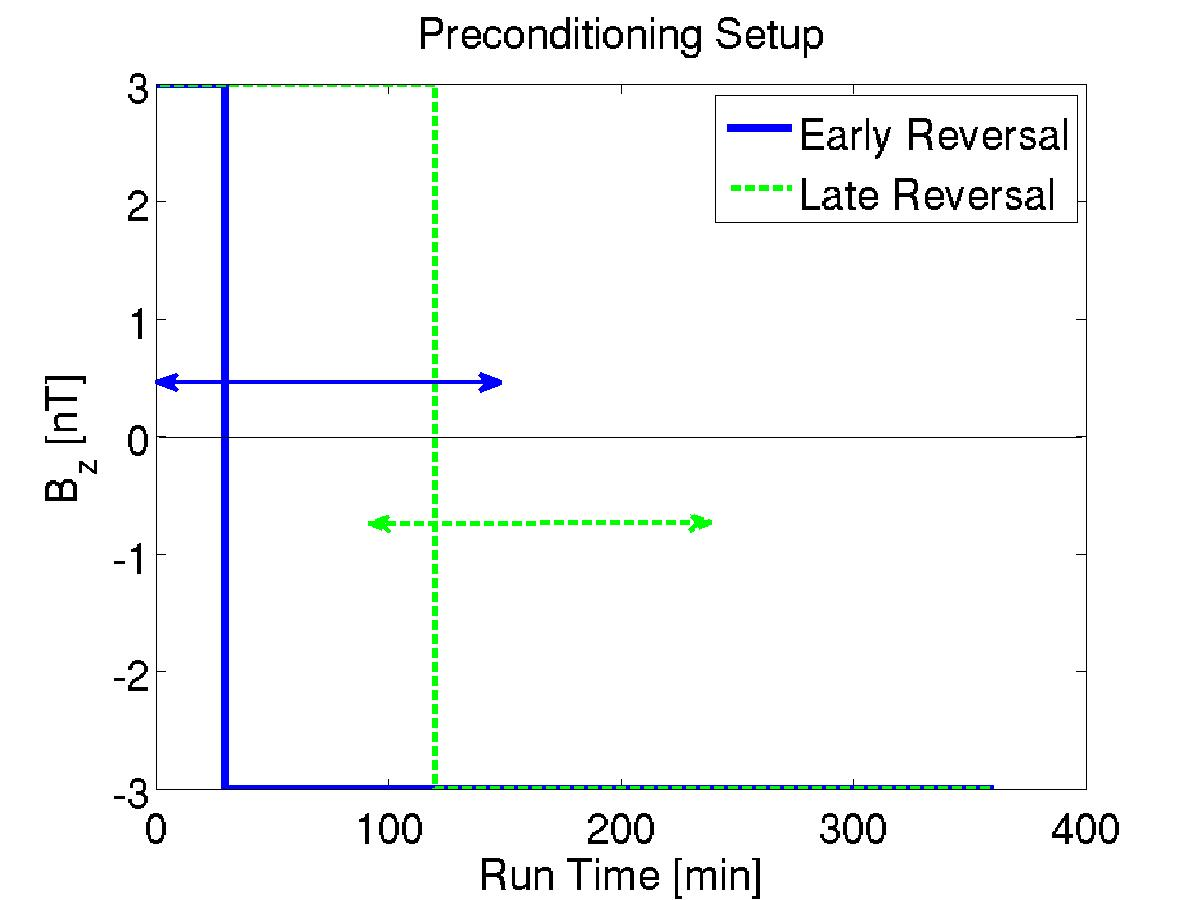
\includegraphics[scale=0.35]{images/PreconditionSetup.jpg}
	\caption{Setup for the preconditioning experiment. Two equal length time
	intervals from each run with the reversal starting at 30 minutes into the start
	of the interval.}
	\label{fig:PreconditionSetup}
	\end{centering}
	\figSpace
\end{figure}

To evaluate the differences between the two models with a time-shifted
$B_z^{IMF}$ reversal, the output data from the two models were taken between 30
minutes before the reversal to 2 hours after the reversal, as shown in Figure
\ref{fig:PreconditionSetup}, and then inserted into the code that creates the
difference output, which was then processed by a Paraview Python code that
creates images.

\begin{table}
\begin{center}
  \caption{Input parameters for preconditioning experiment}
  \begin{tabular}{| l | c | c | c | c | }
    \hline
    \textbf{Run Num.} & \textbf{$\rho$} [$cm^{-3}$] & \textbf{$T$} [$K$] &
    \textbf{$U_x$} [$km/s$] &
    \textbf{$B_z$} [$nT$]
    \\
    \hline 
    1 & 5.76 & 101289 & -442  & +3.1 to -3.0 at 00:30 \\ \hline
    2 & 5.76 & 101289 & -442  & +3.1 to -3.0 at 02:00 \\ \hline
  \end{tabular}
  \label{table:runs12}
\end{center}
\end{table}

As shown in Table \ref{table:runs12} for run 1, $T$, $U_x$, and $\rho$ were kept
constant throughout the entire run. The only difference between the two runs is
the time at which $B_z^{IMF}$ was reversed from a positive to negative value.
This is physically meaningful as a $B_z^{IMF}$ reversal is a typical cause for enhanced
magnetospheric activity.

\subsection{Results}	
% B%
In Figure \ref{fig:BdiffPCBeforeFlip}, the top comparison is between the early
and late reversal runs for the OpenGGCM model. Red indicates locations where
the early reversal has higher values, while blue indicates locations where the
late reversal has higher values. The OpenGGCM model $B_z$ output shows
differences in the positioning of the entire magnetopause with the late reversal
having a magnetopause that is farther Sunward. There are also differences in the
current sheet region with neither the early or late reversal showing
consistently higher or lower values in one specific region of the current sheet.
The BATS-R-US and SWMF models show differences in the current sheet region
between $\pm$ 20 $R_E$ in the z direction.

\begin{figure}
	\centering
	\subfigure{
		\includegraphics[scale=0.36]{/mnt/Disk2/Precondition/Results/0_3/images/Bz_Diff_File1.png}
		}
	\subfigure{
		\includegraphics[scale=0.36]{/mnt/Disk2/Precondition/Results/1_4/images/Bz_Diff_File1.png}
		}
	\subfigure{
		\includegraphics[scale=0.36]{/mnt/Disk2/Precondition/Results/2_5/images/Bz_Diff_File1.png}
		}
	\caption{$B_z$ percent differences between the OpenGGCM model early and late
	reversals (top), BATS-R-US early and late reversals (middle), and SWMF early
	and late reversals (bottom) 25 minutes before the $B_z^{IMF}$ reversal.}
	\figSpace
	\label{fig:BdiffPCBeforeFlip}
\end{figure}

After the $B_z^{IMF}$ reversal, towards the end of the run, there are still
differences in the OpenGGCM model (top) run, while there are minimal to no
differences in the BATS-R-US model (middle) and the SWMF model (bottom) run, as
shown in Figure \ref{fig:BdiffPCAfterFlip}. The differences shown for the OpenGGCM model have
decreased near the magnetopause, but are still large in the current sheet
region.

\begin{figure}
	\centering
	\subfigure{
		\includegraphics[scale=0.36]{/mnt/Disk2/Precondition/Results/0_3/images/Bz_Diff_File26.png}
		}
	\subfigure{
		\includegraphics[scale=0.36]{/mnt/Disk2/Precondition/Results/1_4/images/Bz_Diff_File26.png}
		}
	\subfigure{
		\includegraphics[scale=0.36]{/mnt/Disk2/Precondition/Results/2_5/images/Bz_Diff_File26.png}
		}
	\caption{$B_z$ percent differences between the OpenGGCM model early and late
	reversals (top), BATS-R-US early and late reversals (middle), and SWMF early
	and late reversals (bottom) 60 minutes after the $B_z^{IMF}$ reversal. }
	\figSpace
	\label{fig:BdiffPCAfterFlip}
\end{figure}

% RHO%
In Figure \ref{fig:rhodiffPCBeforeFlip}, the largest differences occur in the
current sheet regions. The OpenGGCM model differences do not extend far
tailward within $\pm$10 $R_E$ in the z direction. The differences in both the BATS-R-US and
SWMF models are highest in the current sheet region and extend into the distant
tail within $\pm$20 $R_E$ in the z direction. In the BATS-R-US model runs, the early
reversal has higher values in the near-Earth current sheet region. In the
SWMF model, the early reversal has higher values nearest Earth outside of the
current sheet region. There are lower values for the late reversal in the
distant tail region.
\begin{figure}
	\centering
	\subfigure{
		\includegraphics[scale=0.36]{/mnt/Disk2/Precondition/Results/0_3/images/rho_Diff_File1.png}
		}
	\subfigure{
		\includegraphics[scale=0.36]{/mnt/Disk2/Precondition/Results/1_4/images/rho_Diff_File1.png}
		}
	\subfigure{
		\includegraphics[scale=0.36]{/mnt/Disk2/Precondition/Results/2_5/images/rho_Diff_File1.png}
		}
	\caption{$\rho$ percent differences between the OpenGGCM model early and late
	reversals (top), BATS-R-US early and late reversals (middle), and SWMF early
	and late reversals (bottom) 25 minutes before the $B_z^{IMF}$ reversal.}
	\figSpace
	\label{fig:rhodiffPCBeforeFlip}
\end{figure}

After the $B_z^{IMF}$ reversal, as shown in Figure \ref{fig:rhodiffPCAfterFlip}, 
there are only small regions of differences in the OpenGGCM model (top). The SWMF
model (bottom), and the BATS-R-US model (middle), have near zero differences.
\begin{figure}
	\centering
	\subfigure{
		\includegraphics[scale=0.36]{/mnt/Disk2/Precondition/Results/0_3/images/rho_Diff_File26.png}
		}
	\subfigure{
		\includegraphics[scale=0.36]{/mnt/Disk2/Precondition/Results/1_4/images/rho_Diff_File26.png}
		}
	\subfigure{
		\includegraphics[scale=0.36]{/mnt/Disk2/Precondition/Results/2_5/images/rho_Diff_File26.png}
		}
	\caption{$\rho$ percent differences between the OpenGGCM model early and late
	reversals (top), BATS-R-US early and late reversals (middle), and SWMF early
	and late reversals (bottom) 60 minutes after the $B_z^{IMF}$ reversal.}
	\figSpace
	\label{fig:rhodiffPCAfterFlip}
\end{figure}

% U_x%
The $U_x$ plots in Figure \ref{fig:UxdiffPCBeforeFlip} show the highest
differences in the current sheet region for all three models.
No one run has higher differences in which the opposite run does
not. The regions in which one run has higher values over the other is not
consistent. The BATS-R-US model (middle) late reversal has highest values in the
current sheet region. The SWMF model (bottom) has highest differences with the
late reversal run in the north and south hemispheres of the magnetosphere outside of
the current sheet region and far from Earth, while the early reversal has higher values
close to Earth.
\begin{figure}
	\centering
	\subfigure{
		\includegraphics[scale=0.36]{/mnt/Disk2/Precondition/Results/0_3/images/Ux_Diff_File1.png}
		}
	\subfigure{
		\includegraphics[scale=0.36]{/mnt/Disk2/Precondition/Results/1_4/images/Ux_Diff_File1.png}
		}
	\subfigure{
		\includegraphics[scale=0.36]{/mnt/Disk2/Precondition/Results/2_5/images/Ux_Diff_File1.png}
		}
	\caption{$\rho$ percent differences between the OpenGGCM model early and late
	reversals (top), BATS-R-US early and late reversals (middle), and SWMF early
	and late reversals (bottom) 25 minutes before the $B_z^{IMF}$ reversal.}
	\figSpace
	\label{fig:UxdiffPCBeforeFlip}
\end{figure}

After the $B_z^{IMF}$ reversal, as shown in Figure \ref{fig:UxdiffPCAfterFlip}, most
of the OpenGGCM model (top) differences are in the current sheet region. The early
reversal has higher values tailward of -40$R_E$, while the late reversal has higher
values Earthward of -40$R_E$.
\begin{figure}
	\centering
	\subfigure{
		\includegraphics[scale=0.36]{/mnt/Disk2/Precondition/Results/0_3/images/Ux_Diff_File26.png}
		}
	\subfigure{
		\includegraphics[scale=0.36]{/mnt/Disk2/Precondition/Results/1_4/images/Ux_Diff_File26.png}
		}
	\subfigure{
		\includegraphics[scale=0.36]{/mnt/Disk2/Precondition/Results/2_5/images/Ux_Diff_File26.png}
		}
	\caption{$\rho$ percent differences between the OpenGGCM model early and late
	reversals (top), BATS-R-US early and late reversals (middle), and SWMF early
	and late reversals (bottom) 60 minutes after the $B_z^{IMF}$ reversal.}
	\figSpace
	\label{fig:UxdiffPCAfterFlip}
\end{figure}

\subsection{Discussion and Conclusions}
The differences in the magnetopause position, for
all three models, are of concern to forecasters. If there is any risk of
the magnetopause traveling farther towards Earth than geosynchronous orbit, then the companies
that control space based technology may need to take action to protect their
equipment from plasma in the solar wind.

The differences seen with all three models, for all three scalar plots, before
the $B_z^{IMF}$ reversal, show that under northward IMF conditions, the model output depends strongly on preconditioning time. With a different output from the same model, there
is an expectation that this would change the effects that the $B_z^{IMF}$ reversal has
on each model under non-artificial conditions. This preconditioning result is similar to results seen with each event validity
validation done where each result is different because the conditions before
$B_z^{IMF}$ reversals were different, as seen in a study by \citet{Juusola2013}.

After the $B_z^{IMF}$ reversal, all three models had smaller differences. The BATS-R-US and SWMF
models both show a decrease of difference to near zero percent. The OpenGGCM
model was the exception in the current sheet region.

In determining if these models had enough preconditioning, the evidence from
this research shows a significant sensitivity to preconditioning time before the
$B_z^{IMF}$ reversal and much smaller differences after the $B_z^{IMF}$
reversal.

\subsubsection{Summary}
\begin{itemize}
  \item Longer preconditioning time allowed the magnetosphere to relax more
  giving different positions for the magnetopause with all three models.
  \item The OpenGGCM model magnetopause position differences were larger than
  that of SWMF or BATS-R-US.
  \item There were large differences for all three models before the $B_z^{IMF}$
  reversal.
  \item The differences in the current sheet region for the OpenGGCM model were similar before and after the reversal.
  \item The BATS-R-US and SWMF model differences decreased after the $B_z^{IMF}$
  reversal to near zero.
\end{itemize}
